\chapter{Example Generator Implementations}
To illustrate a few possibilities of BAG generators, we show various circuits of increasing complexity. 
\section{Starting Small: Passive Loaded Differential Amplifier}
A very commonly used block in many ICs is the differential amplifier. In the case the load is passive. The topology is the same as that used in Chapter 4, and can be seen in section 4.4. An example instance is shown in \ref{fig:passive_amp}.
\begin{figure}[h]
\centering
\begin{subfigure}{.8\linewidth}
  \centering
  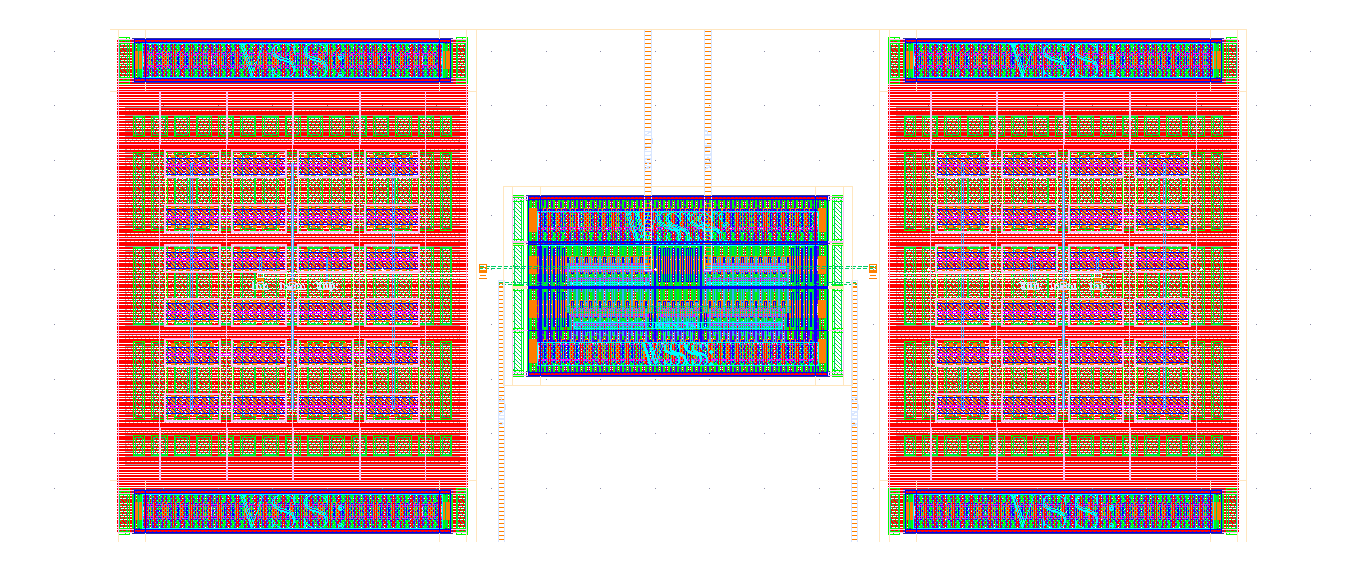
\includegraphics[width=\textwidth]{passive_layout}
  \caption{Full layout}
  \label{fig:sfig1}
\end{subfigure}
\begin{subfigure}{.8\linewidth}
  \centering
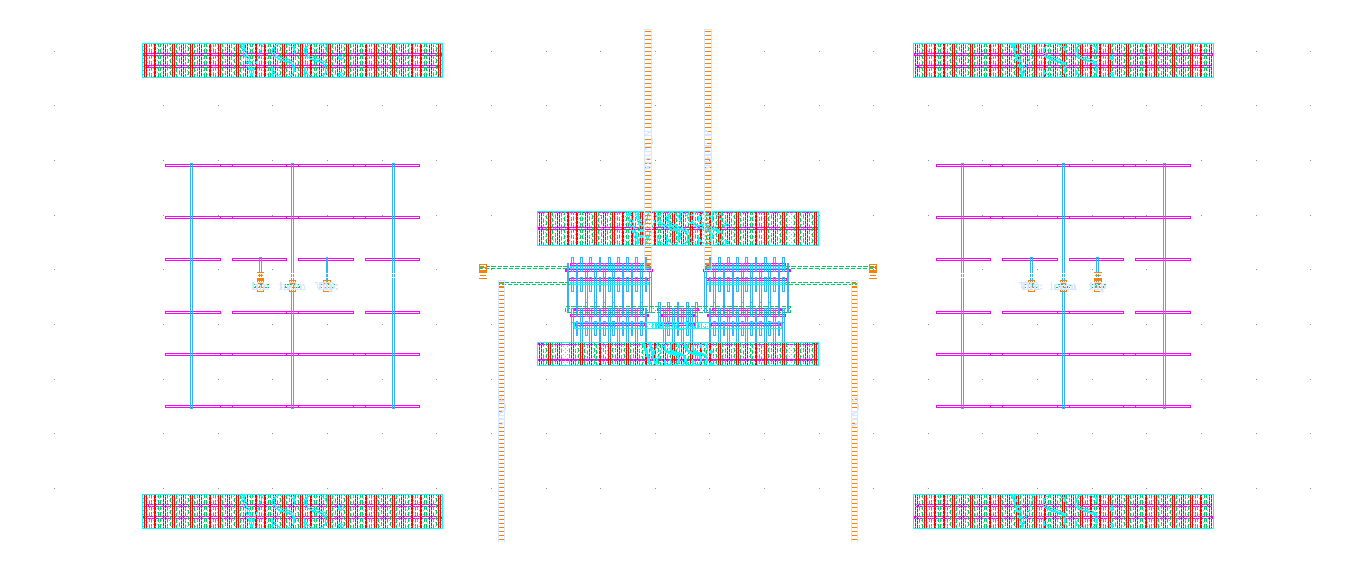
\includegraphics[width=\textwidth]{passive_layout_metals}
  \caption{Only the metals}
  \label{fig:sfig2}
\end{subfigure}
\caption{Differential amplifier layout}
\label{fig:passive_amp}
\end{figure}
\clearpage
All generators demonstrated have wire width parametrized so each type of wire (signal, bias, clock) can have a specific, customizable width. This generator additionally allows the user to specify resistor unit cell sizes, number of parallel and series units and transistor dimensions (width, fingers).

Another option is nearly identical, but with 3-bit resistor DACs instead of a single resistor as in \ref{fig:passive_dac}
\begin{figure}[h]
\centering
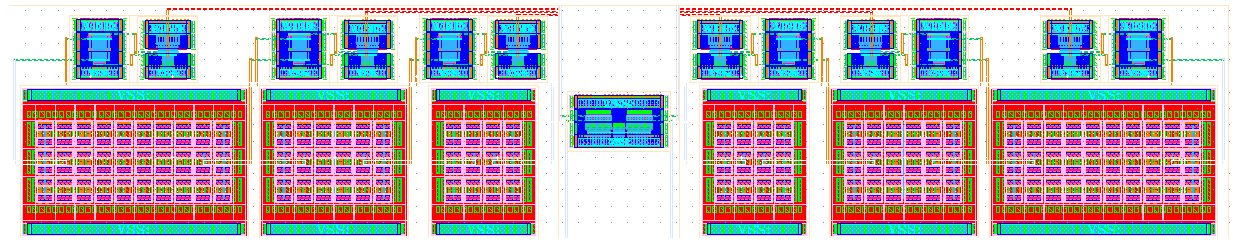
\includegraphics[width=\textwidth]{passive_dac}
\caption{Passive diff-amp with resistor DAC}
\label{fig:passive_dac}
\end{figure}
%\begin{figure}\centering
%\parbox{.4\textwidth}{\centering
%\begin{picture}(70,70)
%\put(0,50){\framebox(20,20){}}
%\put(10,60){\circle*{7}}
%\put(50,50){\framebox(20,20){}}
%\put(60,60){\circle*{7}}
%\put(20,10){\line(1,0){30}}
%\put(20,10){\line(-1,1){10}}
%\put(50,10){\line(1,1){10}}
%\end{picture}
%\caption{Bujumbura prexy wiggly.}}
%\hfill
%\parbox{.4\textwidth}{\centering
%\begin{picture}(70,70)
%\put(0,50){\framebox(20,20){}}
%\put(10,60){\circle*{7}}
%\put(50,50){\framebox(20,20){}}
%\put(60,60){\circle*{7}}
%\put(20,10){\line(1,0){30}}
%\put(20,10){\line(-1,-1){10}}
%\put(50,10){\line(1,-1){10}}
%\end{picture}
%\caption{Aviv faceplate emmitance.}}
%\end{figure}


\section{Getting Fancier: A Double Tail Sense Amplifier and Latch}

Yet another crucial compoenent in an analog reciever is the sampler. Before converting to purely digital processing, the recieved bits must be processed as either a 1 or a 0 through the use of a sampling circuit. While there are many ways to implement sampling, this report makes use of a double tail sense amp (DTSA). The schematic and operation are shown in Chapter 4. An example layout is shown in \ref{fig:dtsa_ex}.
\begin{figure}[h]
\centering
\begin{subfigure}{.4\linewidth}
  \centering
  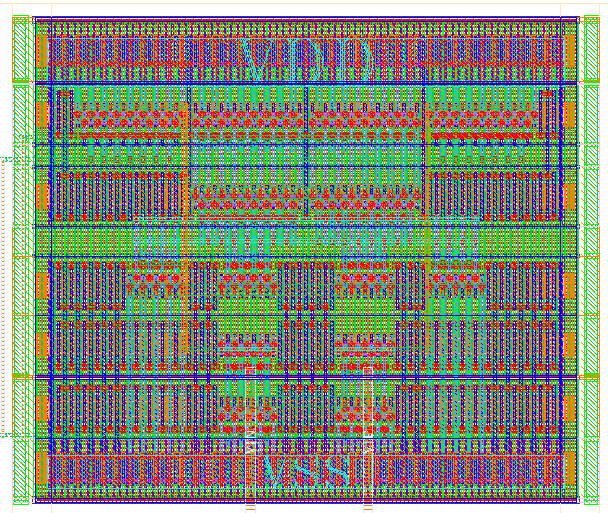
\includegraphics[width=0.8\textwidth]{dtsa_full}
  \caption{Full layout}
  \label{fig:sfig1}
\end{subfigure}
\begin{subfigure}{.4\linewidth}
  \centering
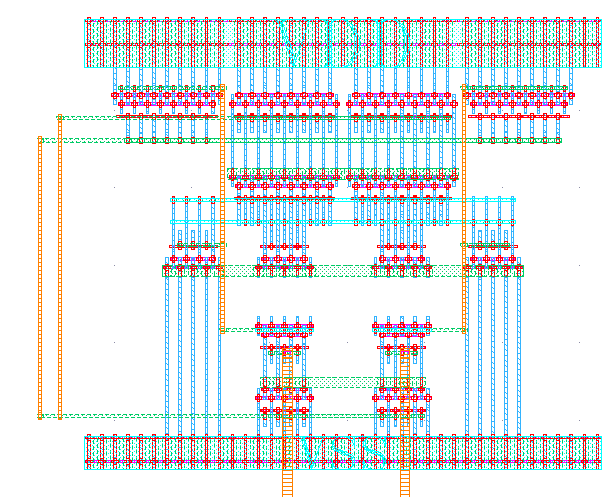
\includegraphics[width=0.8\textwidth]{dtsa_metal}
  \caption{Only the metals}
  \label{fig:sfig2}
\end{subfigure}
\caption{DTSA layout}
\label{fig:dtsa_ex}
\end{figure}
The DTSA block exemplifies even more of BAGs capability to include customization. In addition to all previously mentioned parametrization (wire widths, transistor sizings, etc.) this block also includes an option to generate input pair offset correction hardware. This hardware is implemented as a current that subtracts from the input pair's current during the integration step of operation (discussed more in  Chapter 4). The generator automatically accounts for how the setup changes when offset correction is included, as shown in \ref{fig:dtsa_enoc}.
\begin{figure}[h]
\centering
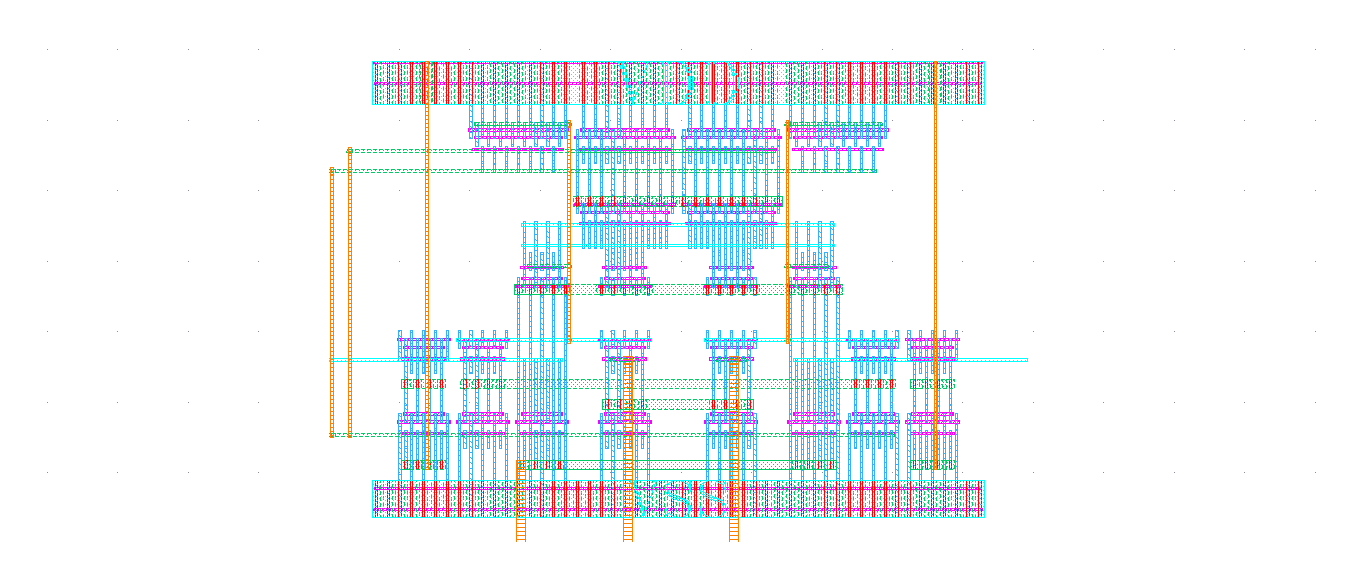
\includegraphics[width=\textwidth]{dtsa_metal_enoc}
\caption{DTSA with offset correction}
\label{fig:dtsa_enoc}
\end{figure}


\section{Endless Possibilities: An Entire Analog Front End Reciever or Two}

Conformance and pave.  Industrial compline dunk transept edifice
downstairs.  Sextillion.  Canvas?  Lyricism webbing insurgent
anthracnose treat familiar.  Apocalyptic quasar; ephemerides
circumstantial.

Peridotite giblet knot.  Navigable aver whee sheath bedraggle twill
era scourge insert.  Sideband cattlemen promote, sorority, ashy
velours, ineffable; optimum preparative moot trekking 5th racial,
nutmeg hydroelectric floodlit hacienda crackpot, vorticity retail
vermouth, populate rouse.  Ceremony?  Fungoid.